\ifx\allfiles\undefined

	% 如果有这一部分另外的package,在这里加上
	% 没有的话不需要
	
	\begin{document}
\else
\fi
    \chapter{图论初步}
    \section{图的基本概念}
	下面给出一些基本的图的概念,注意以下定义并非严格的数学定义,但后续我们将使用以下概念。
	\begin{dfnbox}{图}{}
		由一些点及一些点之间的连线(不带箭头或带箭头)所组成的。一些图中连线的两点无先后次序或重要性差别,而另一些则必须反映这种差别,通常带箭头的连线表示这种差别。
	\end{dfnbox}
	\begin{dfnbox}{边、弧}{}
		不带箭头的连线称为\textbf{边},带箭头的连线称为\textbf{弧}。
	\end{dfnbox}
	\begin{dfnbox}{无向图、有向图}{}
		如果一个图 \( G \) 是由点及边所构成的,则称之为\textbf{无向图}(也简称为\textbf{图}),记为 \( G = (V, E) \),式中 \( V, E \) 分别是 \( G \) 的\textbf{点集合}和\textbf{边集合}。一条连结点 \( vi, vj \in V \) 的边记为 \( [vi, vj] \)(或 \( [vj, vi] \))。如果一个图 \( D \) 是由点及弧所构成的,则称为\textbf{有向图},记为 \( D = (V, A) \),式中 \( V, A \) 分别表示 \( D \) 的\textbf{点集合}和\textbf{弧集合}。一条方向是从 \( vi \) 指向 \( vj \) 的弧记为 \( (vi, vj) \)。
	\end{dfnbox}
	\begin{dfnbox}{点数、边数、弧数}{}
		图 \( G \) 或 \( D \) 中的\textbf{点数}记为 \( p(G) \) 或 \( p(D) \),\textbf{边(弧)数}记为 \( q(G) \)(\( q(D) \))。在不会引起混淆的情况下,也分别简记为 \( p, q \)。
	\end{dfnbox}
	\begin{dfnbox}{端点、环、多重边}{}
		\begin{itemize}
			\item 若边 \( e = [u, v] \in E \),则称 \( u, v \) 是 \( e \) 的\textbf{端点},也称 \( u, v \) 是\textbf{相邻的}。称 \( e \) 是点 \( u \)(及点\( v \))的\textbf{关连边}。
			\item 若图 \( G \) 中,某个边 \( e \) 的两个端点相同,则称 \( e \) 是\textbf{环}。
			\item 若两个点之间有多于一条的边,称这些边为\textbf{多重边}。
			\item 一个无环,无多重边的图称为\textbf{简单图}。
			\item 一个无环,但允许有多重边的图称为\textbf{多重图}。
		\end{itemize}
	\end{dfnbox}
	\begin{dfnbox}{次、悬挂点、奇点}{}
		以点 \( v \) 为端点的边的个数称为 \( v \) 的\textbf{次},记为 \( dG(v) \) 或 \( d(v) \)。环在计算时算作\textcolor{red}{两次}。
		称次为1的点为\textbf{悬挂点},悬挂点的关连边称为\textbf{悬挂边},次为零的点称为\textbf{孤立点}。
		次为奇数的点,称为\textbf{奇点},否则称为\textbf{偶点}。
	\end{dfnbox}
	\begin{dfnbox}{链、圈、初等链、初等圈}{}
		给定一个图 \( G = (V, E) \),一个点、边的交错序列 \((vi1, ei1, vi2, ei2, \cdots, vik-1, eik-1, vik)\),如果满足 \( eit = [vit, vit+1] \) (\( t=1, 2, \cdots, k-1 \)),则称一条联结 \( vi1 \) 和 \( vik \) 的\textbf{链},记为 \((vi1, vi2, \cdots, vik)\),\( vi2, vi3, \cdots, vik-1 \) 为链的\textbf{中间点}。
		链 \((vi1, vi2, \cdots, vik)\) 中,若 \( vi1 = vik \),则称之为一个\textbf{圈},记为 \((vi1, vi2, \cdots, vik-1, vi1)\)。
		若链 \((vi1, vi2, \cdots, vik)\) 中,点 \( vi1, vi2, \cdots, vik \) 都是不同的,则称之为\textbf{初等链};若圈 \((vi1, vi2, \cdots, vik-1, vi1)\) 中,\( vi1, vi2, \cdots, vik-1 \) 都是不同的,则称之为\textbf{初等圈}。
		若链(圈)中含的边均不相同,则称之为\textbf{简单链(圈)}。
	\end{dfnbox}
	\begin{dfnbox}{连通图}{}
		图 \( G \) 中,若任何两个点之间,至少有一条链,则称 \( G \) 是\textbf{连通图},否则称为\textbf{不连通图}。
	\end{dfnbox}
	\begin{dfnbox}{支撑子图}{}
		设一个图 \( G = (V, E) \),如果图 \( G' = (V', E') \),使 \( V' = V \) 及 \( E' \subseteq E \)\footnote{点全部包含,边只包含一部分},则称 \( G' \) 是 \( G \) 的一个\textbf{支撑子图}。
	\end{dfnbox}
	\begin{dfnbox}{基础图}{}
		设有向图 \( D = (V, A) \),从 \( D \) 中去掉所有弧上的箭头,就得到一个无向图,称之为 \( D \) 的\textbf{基础图},记之为 \( G(D) \)。
	\end{dfnbox}
	\begin{dfnbox}{弧的始点与终点}{}
	给 \( D \) 中的一条弧 \( a = (u, v) \),称 \( u \) 为 \( a \) 的\textbf{始点},\( v \) 为 \( a \) 的\textbf{终点},称弧 \( a \) 是从 \( u \) 指向 \( v \) 的。
	设 \( (vi1, ai1, vi2, ai2, \ldots, vik-1, aik-1, vik) \) 是 \( D \) 中的一个点弧交错序列,如果这个序列在基础图 \( G(D) \) 中所对应的点边序列是一条链,则称这个点弧交错序列是 \( D \) 的一条\textbf{链}。
	\end{dfnbox}
	\begin{dfnbox}{路、回路}{}
	如果 \( (vi1, ai1, vi2, ai2, \ldots, vik-1, aik-1, vik) \) 是 \( D \) 中的一条链,并且对 \( t = 1, 2, \ldots, k-1 \),均有 \( ait = (vit, vit+1) \),称之为从 \( vi1 \) 到 \( vik \) 的一条\textbf{路}。若路的第一个点和最后一点相同,则称之为\textbf{回路}。
	\end{dfnbox}



	\section{树}
	\subsection{树和支撑树的概念}
	\begin{dfnbox}{树}{}
		一个无圈的连通图称为\textbf{树}。如:目录树。
		\end{dfnbox}
	\begin{dfnbox}{支撑树}{}
		设图 \( T = (V, E') \) 是图 \( G = (V, E) \) 的支撑子图,如果图 \( T = (V, E') \) 是一个树,则称 \( T \) 是 \( G \) 的一个\textbf{支撑树}。
	\end{dfnbox}
	\begin{itemize}
		\item \textbf{性质}
		\begin{itemize}
			\item \textbf{性质1}:设图 \( G=(V,E) \) 是一个树,\( p(G) \geq 2 \),则 \( G \) 中至少有两个悬点(次为1的点)。
			\item \textbf{性质2}:图 \( G=(V,E) \) 是一个树的充分必要条件是 \( G \) 不含圈,且恰有 \( p-1 \) 条边。即 \( q(G)=p(G)-1 \)。
			\item \textbf{性质3}:图 \( G=(V,E) \) 是一个树的充分必要条件是 \( G \) 是连通图,并且 \( q(G)=p(G)-1 \)。
			\item \textbf{性质4}:图 \( G \) 是树的充分必要条件是任意两个顶点之间恰有一条链。
			\item \textbf{性质5}:图 \( G \) 有支撑树的充分必要条件是图 \( G \) 是连通的。
		\end{itemize}
		\item \textbf{推论}
		\begin{itemize}
			\item \textbf{推论1}:从一个树中去掉任意一条边,则余下的图是不连通的。
			\item \textbf{推论2}:在树中不相邻的两个点间添上一条边,则恰好得到一个圈,如果再从这个圈上任意去掉一条边,可以得到一个树。
		\end{itemize}
	\end{itemize}
	
	那么,如何求一个圆的支撑树?
	\begin{notebox}\textbf{{求圆的支撑树的方法}}{}
		\begin{enumerate}
			\item \textbf{破圈法}\\
			任取一个圈,从圈中去掉一边,对余下的图重复这个步骤,直到不含圈时为止,即得到一个支撑树。
			\begin{figure}[H]
				\centering
				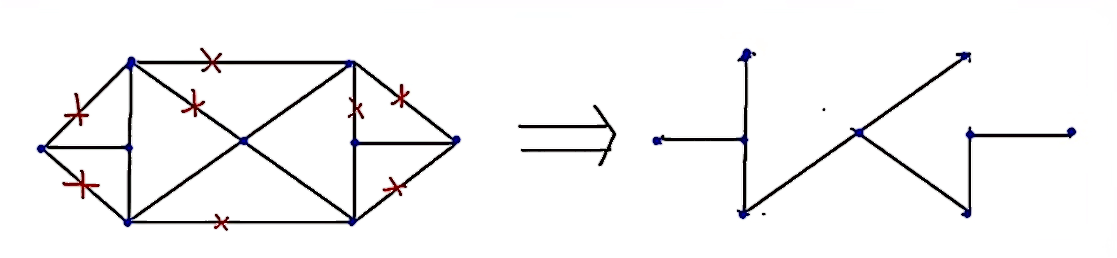
\includegraphics[width=0.8\textwidth]{./image/33.png}
				\caption{破圈法}
				\label{fig:Chapter4_Temporary_Pavilion_1}
			\end{figure}
			\item \textbf{避圈法}\\
			在图中任取一条边e1,找一条与e1不构成圈的边e2,再找一条与{e1,e2}不构成圈的边e3,一般,设已有{e1,e2…,ek},找一条与{e1,e2,…,ek}中的任何一些边不构成圈的边ek+1。重复这个过程,直到不能进行为止。这时,由所有取出的边所构成的图是一个支撑树,称这种方法为“避圈法”
			\begin{figure}[H]
				\centering
				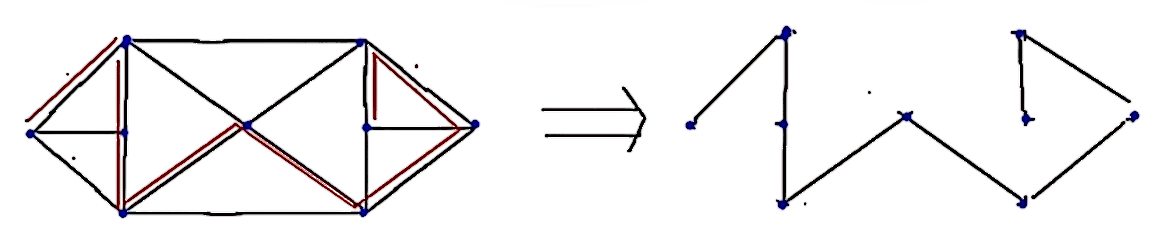
\includegraphics[width=0.8\textwidth]{./image/34.png}
				\caption{避圈法}
				\label{fig:Chapter4_Temporary_Pavilion_1}
			\end{figure}
		\end{enumerate}
	\end{notebox}

	\subsection{最小支撑树问题及其求解}
	\begin{dfnbox}{赋权图}
	给图 \( G = (V, E) \),对 \( G \) 中的每一条边 \([vi, vj]\),相应地有一数 \( w_{ij} \),则称这样的图 \( G \) 为\textbf{赋权图},\( w_{ij} \) 称为边 \([vi, vj]\) 上的\textbf{权}。
	\end{dfnbox}
	\textbf{权的物理含义}:距离、时间、费用等。
	\begin{dfnbox}{最小支撑树}
	如果 \( T = (V, E') \) 是 \( G \) 的一个\textbf{支撑树},称 \( E' \) 中所有边的权之和为支撑树 \( T \) 的\textbf{权},记为 \( W(T) \):
	\[ W(T) = \sum_{[vi,vj]\in E'} w_{ij} \]
	如果支撑树 \( T^* \) 的权 \( W(T^*) \) 是 \( G \) 的所有支撑树的权中最小者,则称 \( T^* \) 是 \( G \) 的\textbf{最小支撑树}(简称\textbf{最小树}):
	\[ W(T^*) = \min_{T} W(T) \]
	\end{dfnbox}
	最小支撑树问题就是求\textcolor{red}{给定连通赋权图G的最小支撑树}。
	\begin{exbox}{电话线网问题}{}
		\textbf{例:}某工厂内联结六个车间的道路网如图所示。已知每条道路的长,要求沿道路架设联结六个车间的电话线网,使电话线的总长最小?
		\begin{figure}[H]
			\centering
			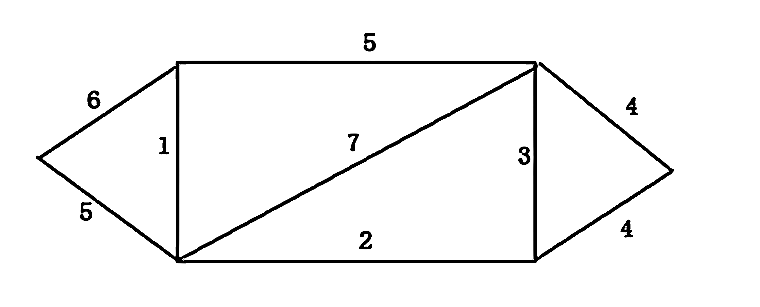
\includegraphics[width=0.7\textwidth]{./image/35.png}
			\caption{工厂道路网图}
			\label{fig:Chapter4_Temporary_Pavilion_1}
		\end{figure}
		\textbf{解:}
		\begin{itemize}
			\item \textbf{破圈法}\\
			任取一个圈,从圈中去掉一条\textcolor{red}{权最大}的边(如果有两条或两条以上的边都是权最大的边,则任意去掉其中一条)\footnote{注意只破除那些仍然在圈中的权重最大的,如果有权重很大但不在任何一个圈内的不必再破除}。在余下的图中,重复这个步骤,直至得到一个不含圈的图为止,这时的图便是最小树。
			\begin{figure}[H]
				\centering
				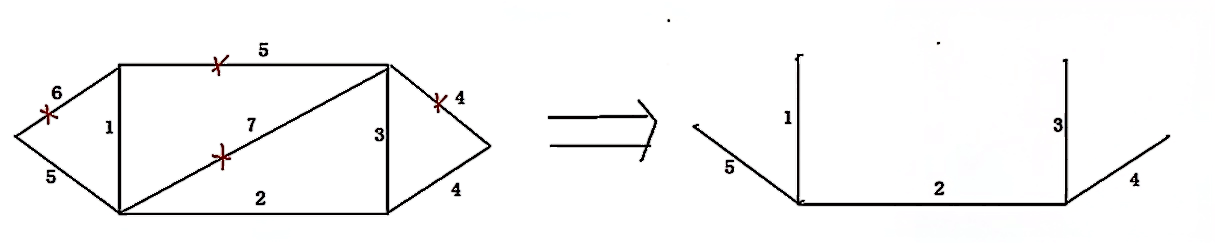
\includegraphics[width=0.7\textwidth]{./image/36.png}
				\caption{破圈法解决电话线问题}
				\label{fig:Chapter4_Temporary_Pavilion_1}
			\end{figure}
			\item \textbf{避圈法}\\
			开始选一条\textcolor{red}{最小}权边,以后每一步中总从未被选中的边中选一条\textcolor{red}{权最小}的边,并不与已选取的边构成圈(若有两条最小权边,则任选一条)
			\begin{figure}[H]
				\centering
				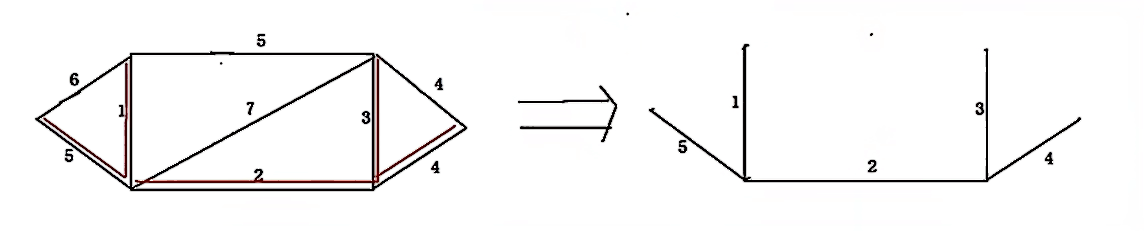
\includegraphics[width=0.7\textwidth]{./image/37.png}
				\caption{避圈法解决电话线问题}
				\label{fig:Chapter4_Temporary_Pavilion_1}
			\end{figure}
		\end{itemize}
	\end{exbox}
	\section{最短路问题}
	\subsection{最短路问题的概念}
	\begin{dfnbox}{最短路问题}{赋权有向图的最短路径}
		给定一个\textbf{赋权有向图} \( D = (V, A) \),其中:
		\begin{itemize}
			\item 对每个弧 \( a = (v_i, v_j) \in A \),有权值 \( W(a) = w_{ij} \)
			\item 给定两个顶点 \( v_s \)(起点)和 \( v_t \)(终点)
		\end{itemize}
		设 \( P \) 是 \( D \) 中从 \( v_s \) 到 \( v_t \) 的一条\textbf{路},定义其\textbf{权值}为:
		\[ W(P) = \sum_{a \in P} W(a) \]
		\textbf{最短路问题}即求解:
		\[ W(P_0) = \min_{P \in \mathcal{P}} W(P) \]
		其中 \( \mathcal{P} \) 表示所有从 \( v_s \) 到 \( v_t \) 的路的集合,\( P_0 \) 称为\textbf{最短路}。
		对应的\textbf{距离}定义为:
		\[ d(v_s, v_t) = W(P_0) \]
		注意:在有向图中,\( d(v_s, v_t) \) 与 \( d(v_t, v_s) \) 不一定相等。
	\end{dfnbox}
	\begin{exbox}{最短路问题}{}
		\textbf{例:}如图所示的单行线交通网,弧上数字为里程。问:从v1出发,通过交通网到v8,哪一条路总里程最小?从v1-v8的路线很多:每条路线里程不同,哪一条最小?
		\begin{figure}[H]
			\centering
			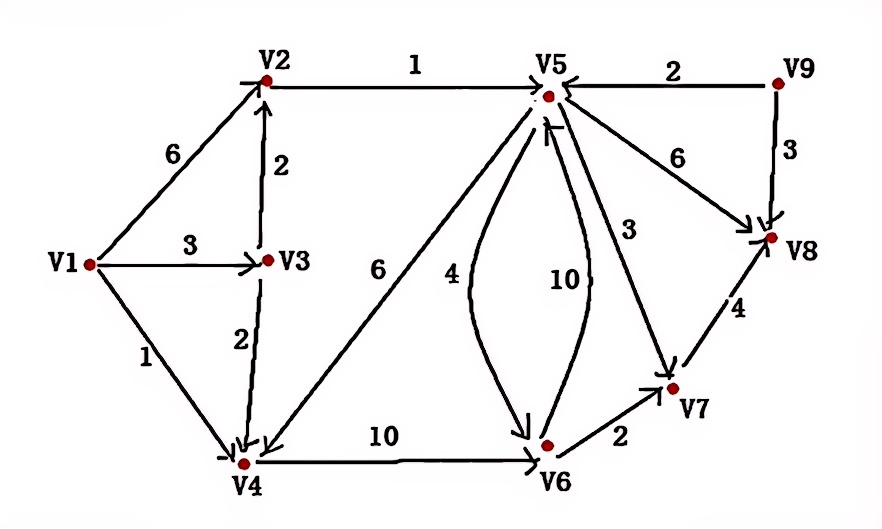
\includegraphics[width=0.7\textwidth]{./image/38.png}
			\caption{单行线交通网图}
			\label{fig:Chapter4_Temporary_Pavilion_1}
		\end{figure}
	\end{exbox}
	\textbf{说明:}
	\begin{enumerate}
		\item 上述距离并非只能指里程,其物理意义可以是费用、时间等其他含义,完全视权的物理含义而定。
		\item 对于无向图,最短路问题依然存在(如推销员旅行问题即为其一个变种),此时称为最短链问题。
	\end{enumerate}

	\subsection{最短路问题的求解:Dijkstra算法}
	\subsubsection{Dijkstra算法的前提和结果适用性}
	\begin{itemize}
		\item 该方法只适用于权$W_{ij} \geq 0$的情况
		\item 该方法不仅求出了从初始点到终点的最短路,实际上它求出了从初始点到任何一点的最短路。
	\end{itemize}
	
	\begin{thmbox}{Dijkstra算法的理论依据}{}
	\begin{itemize}
		\item 最短路最优子结构性质:
		\begin{quote}
			如果 $P$ 是 $D$ 中从 $v_s$ 到 $v_j$ 的最短路,$v_i$ 是 $P$ 上的任一中点,则从 $v_s$ 沿 $P$ 到 $v_i$ 的子路径必为 $v_s$ 到 $v_i$ 的最短路。
		\end{quote}
		\item 反证法证明:
		\begin{itemize}
			\item 假设存在更短的路径 $Q$ 从 $v_s$ 到 $v_i$
			\item 构造新路径 $P' = Q \cup P_{v_i \to v_j}$
			\item 则 $W(P') < W(P)$,与 $P$ 是最短路矛盾
		\end{itemize}
	\end{itemize}
	\begin{figure}[H]
		\centering
		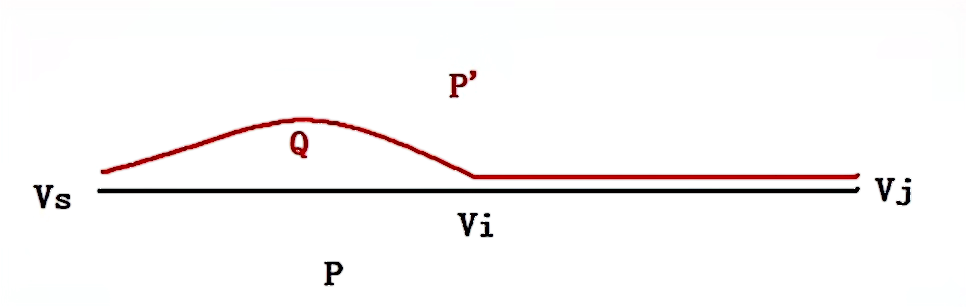
\includegraphics[width=0.7\textwidth]{./image/39.png}
		\caption{反证法证明图}
		\label{fig:Chapter4_Temporary_Pavilion_1}
	\end{figure}
	\end{thmbox}

	\subsubsection{算法思想}
	\begin{itemize}
		\item \textbf{标号类型}:
		\begin{itemize}
			\item 临时标号(T标号):最短路上界,可更新
			\item 永久标号(P标号):最短路权值,不再改变
		\end{itemize}
		\item \textbf{轨迹记录}:
		\begin{itemize}
			\item 定义 $\lambda(v)$ 记录前驱节点
			\item $\lambda(v)=M$ 表示不可达
			\item $\lambda(v)=0$ 表示起点
		\end{itemize}
	\end{itemize}
	\begin{notebox}{\textbf{标号过程}}{}
		\begin{enumerate}[label=第一步:, leftmargin=*]
			\item \textbf{修改T标号}
			
			设$v_i$是新产生的P标号点,考察所有以$v_i$为始点的弧段$v_i \to v_j$:
			\begin{itemize}
				\item 如果$v_j$已经是P标号点,则不再处理
				\item 如果$v_j$是T标号点,则按以下规则更新:
				\[ T(v_j) = \min\left[T(v_j),\ P(v_i) + w_{ij}\right] \]
				其中\footnote{本质上,是让到新的标号点$v_{j}$的“距离”为以前已经确定好的到$v_i$的最短路$P(v_i)$加上弧段$v_i \to v_j$的权值$w_{ij}$,产生若干个$T$,确定最短的那个为新的$P$:即没确定的时候是T,确定了是P。}:
				\begin{itemize}
					\item $T(v_j)$表示$v_j$点旧的T标号值
					\item $w_{ij}$表示弧段$v_i \to v_j$的权值
				\end{itemize}
			\end{itemize}
		\end{enumerate}
		
		\begin{enumerate}[label=第二步:, start=2, leftmargin=*]
			\item \textbf{产生新的P标号}
			
			按照以下原则进行:
			\begin{itemize}
				\item 在所有现有的T标号点中,选择值最小的改为P标号
				\item 重复上述两个步骤,直到终点的T标号变为P标号为止
			\end{itemize}
		\end{enumerate}
	\end{notebox}
	\subsubsection{算法步骤}
	\begin{thmbox}{\textbf{Dijkstra算法}}{}
		\begin{itemize}
		\item {\textbf{符号定义}}
		\begin{itemize}
			\item 用$P(v_i)$、$T(v_j)$分别表示$v_i$点的P标号、T标号
			\item $S_i$表示第$i$步时具有P标号点的集合(其中有已经确定好的走的那些点)
			\item $\lambda(v)$表示轨迹标记,可以回溯父节点,初值$\lambda(v)=M$,其中:
			\begin{itemize}
				\item $\lambda(v)=m$:在$v_s$到$v$的最短路上,$v$的前一个点是$v_m$
				\item $\lambda(v)=M$:$D$中不含从$v_s$到$v$的路(最开始不知道谁是谁的爹,所以统一用M表示)
				\item $\lambda(v)=0$:表示$v=v_s$(第一个节点,父亲竟是我自己)
			\end{itemize}

		\end{itemize}
		
		\item {\textbf{算法流程}}
		\begin{enumerate}[label=\textbf{步骤 \arabic*:}, leftmargin=*]
			\item \textbf{开始} ($i=0$)
			\begin{itemize}
				\item 令P标号集合$S_0 = \{v_s\}$
				\item P标号点的权值$P(v_s) = 0$
				\item 路径标记$\lambda(v_s) = 0$
				\item 对每一个$v \neq v_s$:
				\begin{itemize}
					\item 令T标号权值$T(v) = +\infty$
					\item $\lambda(v) = M$
				\end{itemize}
				\textcolor{red}{即T标号,即未确定的点,权值为无穷大,路径标记为M(不知道爹是谁)}
				\item 令$k = s$($k$为当前最新的P标号点)
			\end{itemize}
			
			\item \textbf{第一步}
			\begin{itemize}
				\item 如果$S_i = V$(全部点的集合),算法终止
				\begin{itemize}
					\item 对每个$v \in S_i$,$d(v_s,v) = P(v)$
				\end{itemize}
				\item 否则转入"第二步"
			\end{itemize}
			
			\item \textbf{第二步}
			\begin{itemize}
				\item 考查每个使$(v_k,v_j) \in A$且$v_j \notin S_i$的点$v_j$(找还没纳入进来的点)
				\item 即考察所有以$v_k$为始点的弧段$v_k \to v_j$(注意只往前走一步)
				\item 如果$T(v_j) > P(v_k) + w_{kj}$,则:
				\begin{itemize}
					\item 把$T(v_j)$修改为$P(v_k) + w_{kj}$
					\item 把$\lambda(v_j)$修改为$k$
				\end{itemize}
				\item 如果$T(v_j) \leq P(v_k) + w_{kj}$,转入"第三步"
			\end{itemize}
			
			\item \textbf{第三步}
			\begin{itemize}
				\item 令$T(v_{j^*}) = \min\limits_{v_j \notin S_i} \{T(v_j)\}$
				\item 在所有现有的T标号中找出值最小的那一个
				\item 如果$T(v_{j^*}) < +\infty$,则:
				\begin{itemize}
					\item 把$v_{j^*}$的T标号变为P标号$P(v_{j^*}) = T(v_{j^*})$
					\item 令$S_{i+1} = S_i \cup \{v_{j^*}\}$
					\item 令$k = j^*$
					\item 把$i$换成$i+1$,转入"第一步"
				\end{itemize}
				\item 否则终止
				\begin{itemize}
					\item 对每一个$v \in S_i$,$d(v_s,v) = P(v)$
					\item 对每一个$v \notin S_i$,$d(v_s,v) = T(v)$(即找不到通路)
				\end{itemize}
			\end{itemize}
		\end{enumerate}
	\end{itemize}
	\end{thmbox}
	\begin{exbox}{续9.3.2:最短路问题}{}
		\textbf{例:}如图所示的单行线交通网,弧上数字为里程。问:从v1出发,通过交通网到v8,哪一条路总里程最小?从v1-v8的路线很多:每条路线里程不同,哪一条最小?
		\begin{figure}[H]
			\centering
			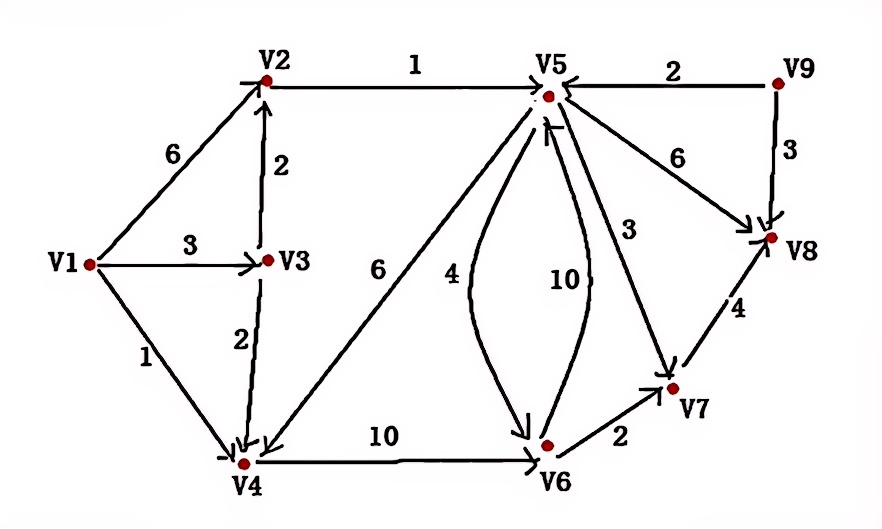
\includegraphics[width=0.7\textwidth]{./image/38.png}
			\caption{单行线交通网图}
			\label{fig:Chapter4_Temporary_Pavilion_1}
		\end{figure}
		\textbf{解:}
		\begin{enumerate}[label=(\arabic*)]
			\item \( i = 0 \).
			\begin{itemize}
				\item 令 \( S_0 = \{v_1\} \), \( P(v_1) = 0 \), \( \lambda(v_1) = 0 \)。
				\item 再令:除 \( v_1 \) 以外的所有其他点,
				\[
				T(v_2) = T(v_3) = T(v_4) = T(v_5) = T(v_6) = T(v_7) = T(v_8) = T(v_9) = +\infty
				\]
				\[
				\lambda(v_2) = \lambda(v_3) = \lambda(v_4) = \lambda(v_5) = \lambda(v_6) = \lambda(v_7) = \lambda(v_8) = \lambda(v_9) = M
				\]
				\item 令 \( k = 1 \)(\( k \) 为当前最新的P标号标号)。
				\item 转入“第二步”,
				\begin{itemize}
					\item \(\because (v_1, v_2) \in A\), \( v_2 \notin S_0 \), \( P(v_1) + w_{12} = 0 + 6 < T(v_2) = +\infty \)
					\item \(\therefore\) 修改 \( T(v_2) \): \( T(v_2) = P(v_1) + w_{12} = 6 \)
					\item 修改 \( \lambda(v_2) \): \( \lambda(v_2) = 1 \)
					\item 同理,修改 \( T(v_3) \) 和 \( \lambda(v_3) \): \( T(v_3) = P(v_1) + w_{13} = 3 \), \( \lambda(v_3) = 1 \)
					\item 修改 \( T(v_4) \) 和 \( \lambda(v_4) \): \( T(v_4) = P(v_1) + w_{14} = 1 \), \( \lambda(v_4) = 1 \)
				\end{itemize}
				\item 转入“第三步”,在所有 \( T \) 标号中比较大小。
				\[
				\min\{T(v_2), T(v_3), T(v_4), T(v_5), T(v_6), T(v_7), T(v_8), T(v_9)\} = T(v_4) = 1
				\]
				\[
				(T(v_2) = 6, T(v_3) = 3, T(v_4) = 1, T(v_5) = T(v_6) = T(v_7) = T(v_8) = T(v_9) = +\infty)
				\]
				\item 令 \( P(v_4) = 1 \), \( S_1 = S_0 \cup \{v_4\} = \{v_1, v_4\} \),且 \( k = 4 \)。
				\item 本步计算结果:
				\begin{itemize}
					\item \( i = 0 \)
					\item \( k = 1, 4 \)
					\item \( S_1 = \{v_1, v_4\} \)
					\item \( P(v_1) = 0 \), \( P(v_4) = 1 \), \( \lambda(v_4) = 1 \)
					\item \( T(v_2) = 6 \), \( T(v_3) = 3 \)
					\item \( \lambda(v_2) = 1 \), \( \lambda(v_3) = 1 \)
					\item \( T(v_5) = T(v_6) = T(v_7) = T(v_8) = T(v_9) = +\infty \)
					\item \( \lambda(v_5) = \lambda(v_6) = \lambda(v_7) = \lambda(v_8) = \lambda(v_9) = M \)
				\end{itemize}
			\end{itemize}
		
			\item \( i = 1 \)
			\begin{itemize}
				\item 转“第二步”,以 \( v_4 \) 为当前始点,考虑所有以 \( v_4 \) 为始点的弧段(只有 \( v_6 \))
				\begin{itemize}
					\item \(\because P(v_4) + w_{46} = 1 + 10 = 11 < T(v_6) = +\infty \)
					\item \(\therefore\) 修改 \( T(v_6) \): \( T(v_6) = P(v_4) + w_{46} = 11 \)
					\item 修改 \( \lambda(v_6) \): \( \lambda(v_6) = 4 \)
				\end{itemize}
				\item 转入“第三步”,所有 \( T \) 标号中比较大小。
				\[
				\min\{T(v_2), T(v_3), T(v_6), T(v_5), T(v_7), T(v_8), T(v_9)\} = T(v_3) = 3
				\]
				\[
				(T(v_2) = 6, T(v_3) = 3, T(v_6) = 11, T(v_5) = T(v_7) = T(v_8) = T(v_9) = +\infty)
				\]
				\item 令 \( P(v_3) = 3 \), \( S_2 = S_1 \cup \{v_3\} = \{v_1, v_4, v_3\} \),且 \( k = 3 \)。
				\item 本步计算结果:
				\begin{itemize}
					\item \( i = 1 \)
					\item \( k = 1, 4, 3 \)
					\item \( S_2 = \{v_1, v_4, v_3\} \)
					\item \( P(v_1) = 0 \), \( P(v_4) = 1 \), \( \lambda(v_4) = 1 \)
					\item \( P(v_3) = 3 \), \( \lambda(v_3) = 1 \)
					\item \( T(v_2) = 6 \), \( T(v_6) = 11 \)
					\item \( \lambda(v_2) = 1 \), \( \lambda(v_6) = 4 \)
					\item \( T(v_5) = T(v_7) = T(v_8) = T(v_9) = +\infty \)
					\item \( \lambda(v_5) = \lambda(v_7) = \lambda(v_8) = \lambda(v_9) = M \)
				\end{itemize}
			\end{itemize}
		
			\item \( i = 2 \)
			\begin{itemize}
				\item 转“第二步”,以 \( v_3 \) 为当前始点,考察所有以 \( v_3 \) 为始点的弧段 \( (v_3, v_2) \) 和 \( (v_3, v_4) \)。
				\begin{itemize}
					\item \(\because v_1 \) 已经 \( \in S_2 \),\textcolor{red}{不用再考察 \( (v_3, v_4) \),只考察 \( v_2 \) 即可}。
					\item \(\because P(v_3) + w_{32} = 3 + 2 = 5 < T(v_2) = 6 \)
					\item \(\therefore\) 修改 \( T(v_2) \): \( T(v_2) = P(v_3) + w_{32} = 5 \)
					\item 修改 \( \lambda(v_2) \): \( \lambda(v_2) = 3 \)
				\end{itemize}
				\item 转入“第三步”,所有 \( T \) 标号中比较大小。
				\[
				\min \{T(v_2), T(v_6), T(v_5), T(v_7), T(v_8), T(v_9)\} = T(v_2) = 5
				\]
				\[
				(T(v_2) = 5, T(v_6) = 11, T(v_5) = T(v_7) = T(v_8) = T(v_9) = +\infty)
				\]
				\item 令 \( P(v_2) = 5 \), \( S_3 = S_2 \cup \{v_2\} = \{v_1, v_4, v_3, v_2\} \),且 \( k = 2 \)。
				\item 本步计算结果:
				\begin{itemize}
					\item \( i = 2 \)
					\item \( k = 1, 4, 3, 2 \)
					\item \( S_3 = \{v_1, v_4, v_3, v_2\} \)
					\item \( P(v_1) = 0 \), \( P(v_4) = 1 \), \( \lambda(v_4) = 1 \)
					\item \( P(v_3) = 3 \), \( \lambda(v_3) = 1 \)
					\item \( P(v_2) = 5 \), \( \lambda(v_2) = 3 \)
					\item \( T(v_6) = 11 \), \( \lambda(v_6) = 4 \)
					\item \( T(v_5) = T(v_7) = T(v_8) = T(v_9) = +\infty \)
					\item \( \lambda(v_5) = \lambda(v_7) = \lambda(v_8) = \lambda(v_9) = M \)
				\end{itemize}
			\end{itemize}
		
			\item \( i = 3 \)
			\begin{itemize}
				\item 转“第二步”,以 \( v_2 \) 为当前始点,考察所有以 \( v_2 \) 为始点的弧段,只有 \( v_5 \)。
				\begin{itemize}
					\item \(\because P(v_2) + w_{25} = 5 + 1 = 6 < T(v_5) = +\infty \)
					\item \(\therefore\) 修改 \( T(v_5) \): \( T(v_5) = P(v_2) + w_{25} = 6 \)
					\item 修改 \( \lambda(v_5) \): \( \lambda(v_5) = 2 \)
				\end{itemize}
				\item 转入“第三步”,所有 \( T \) 标号中比较大小。
				\[
				\min\{T(v_5), T(v_6), T(v_7), T(v_8), T(v_9)\} = T(v_5) = 6
				\]
				\[
				(T(v_5) = 6, T(v_6) = 11, T(v_7) = T(v_8) = T(v_9) = +\infty)
				\]
				\item 令 \( P(v_5) = 6 \), \( S_4 = S_3 \cup \{v_5\} = \{v_1, v_4, v_3, v_2, v_5\} \),且 \( k = 5 \)。
				\item 本步计算结果:
				\begin{itemize}
					\item \( i = 3 \)
					\item \( k = 1, 4, 3, 2, 5 \)
					\item \( S_4 = \{v_1, v_4, v_3, v_2, v_5\} \)
					\item \( P(v_1) = 0 \), \( P(v_4) = 1 \), \( \lambda(v_4) = 1 \)
					\item \( P(v_3) = 3 \), \( \lambda(v_3) = 1 \)
					\item \( P(v_2) = 5 \), \( \lambda(v_2) = 3 \)
					\item \( P(v_5) = 6 \), \( \lambda(v_5) = 2 \)
					\item \( T(v_6) = 11 \), \( \lambda(v_6) = 4 \)
					\item \( T(v_7) = T(v_8) = T(v_9) = +\infty \)
					\item \( \lambda(v_7) = \lambda(v_8) = \lambda(v_9) = M \)
				\end{itemize}
			\end{itemize}
		
			\item \( i = 4 \)
			\begin{itemize}
				\item 转“第二步”,以 \( v_5 \) 为当前始点,考察所有后继结点为 \( v_4, v_6, v_7, v_8 \)。
				\begin{itemize}
					\item \(\because v_4 \) 已经 \( \in S_4 \),只考察 \( v_6, v_7, v_8 \)。
					\item \(\because P(v_5) + w_{56} = 6 + 4 = 10 < T(v_6) = 11 \)
					\item \(\therefore\) 修改 \( T(v_6) \): \( T(v_6) = P(v_6) + w_{56} = 10 \)
					\item 修改 \( \lambda(v_6) \): \( \lambda(v_6) = 5 \)
					\item 同理:
					\begin{itemize}
						\item 修改 \( T(v_7) \): \( T(v_7) = P(v_5) + w_{57} = 6 + 3 = 9 \), \( \lambda(v_7) = 5 \)
						\item 修改 \( T(v_8) \): \( T(v_8) = P(v_5) + w_{58} = 6 + 6 = 12 \), \( \lambda(v_8) = 5 \)
					\end{itemize}
				\end{itemize}
				\item 转入“第三步”,所有 \( T \) 标号中比较大小。
				\[
				\min \{T(v_6), T(v_7), T(v_8), T(v_9)\} = T(v_7) = 9
				\]
				\[
				(T(v_6) = 10, T(v_7) = 9, T(v_8) = 12, T(v_9) = +\infty)
				\]
				\item 令 \( P(v_7) = 9 \), \( S_5 = S_4 \cup \{v_7\} = \{v_1, v_4, v_3, v_2, v_5, v_7\} \),且 \( k = 7 \)。
				\item 本步计算结果:
				\begin{itemize}
					\item \( i = 4 \)
					\item \( k = 1, 4, 3, 2, 5, 7 \)
					\item \( S_4 = \{ v_1, v_4, v_3, v_2, v_5, v_7 \} \)
					\item \( P(v_1) = 0 \), \( P(v_4) = 1 \), \( \lambda(v_4) = 1 \)
					\item \( P(v_3) = 3 \), \( \lambda(v_3) = 1 \)
					\item \( P(v_2) = 5 \), \( \lambda(v_2) = 3 \)
					\item \( P(v_5) = 6 \), \( \lambda(v_5) = 2 \)
					\item \( P(v_7) = 9 \), \( \lambda(v_7) = 5 \)
					\item \( T(v_6) = 10 \), \( \lambda(v_6) = 5 \)
					\item \( T(v_8) = 12 \), \( \lambda(v_8) = 5 \)
					\item \( T(v_9) = +\infty \), \( \lambda(v_9) = M \)
				\end{itemize}
			\end{itemize}
			\item \( i = 5 \)
    \begin{itemize}
        \item 转“第二步”,以 \( v_7 \) 为当前始点,考察所有后继结点:只有 \( v_8 \)。
        \[
        P(v_7) + w_{78} = 9 + 4 = 13 > T(v_8) = 12
        \]
        \begin{itemize}
            \item \textcolor{red}{故 \( T(v_8) \) 不变,\( \lambda(v_8) \) 不变}。
        \end{itemize}
        \item 转入“第三步”,所有 \( T \) 标号中比较大小。
        \[
        \min\{T(v_6), T(v_8), T(v_9)\} = T(v_6) = 10
        \]
        \[
        (T(v_6) = 10, T(v_8) = 12, T(v_9) = +\infty)
        \]
        \item 令 \( P(v_6) = 10 \), \( S_6 = S_5 \cup \{v_6\} = \{v_1, v_4, v_3, v_2, v_5, v_7, v_6\} \),且 \( k = 6 \)。
        \item 本步计算结果:
        \begin{itemize}
            \item \( i = 5 \)
            \item \( k = 1, 4, 3, 2, 5, 7, 6 \)
            \item \( S_4 = \{v_1, v_4, v_3, v_2, v_5, v_7, v_6\} \)
            \item \( P(v_1) = 0 \), \( P(v_4) = 1 \), \( \lambda(v_4) = 1 \)
            \item \( P(v_3) = 3 \), \( \lambda(v_3) = 1 \)
            \item \( P(v_2) = 5 \), \( \lambda(v_2) = 3 \)
            \item \( P(v_5) = 6 \), \( \lambda(v_5) = 2 \)
            \item \( P(v_7) = 9 \), \( \lambda(v_7) = 5 \)
            \item \( P(v_6) = 10 \), \( \lambda(v_6) = 5 \)
            \item \( T(v_8) = 12 \), \( \lambda(v_8) = 5 \)
            \item \( T(v_9) = +\infty \), \( \lambda(v_9) = M \)
        \end{itemize}
    \end{itemize}

    \item \( i = 6 \)
    \begin{itemize}
        \item 转“第二步”,以 \( v_6 \) 为当前始点,考察所有后继结点:\( v_5 \)、\( v_7 \)。
        \begin{itemize}
            \item \( v_5 \),\( v_7 \) 已经 \( \in S_6 \),直接转“第三步”。
        \end{itemize}
        \item 转入“第三步”,所有 \( T \) 标号中比较大小。
        \[
        \min\{T(v_8), T(v_9)\} = T(v_8) = 12
        \]
        \[
        (T(v_8) = 12, T(v_9) = +\infty)
        \]
        \item 令 \( P(v_8) = 12 \), \( S_7 = S_6 \cup \{v_8\} = \{v_1, v_4, v_3, v_2, v_5, v_7, v_6, v_8\} \),且 \( k = 8 \)。
        \item 至此,目标已达到。
        \item 本步计算结果:
        \begin{itemize}
            \item \( i = 6 \)
            \item \( k = 1, 4, 3, 2, 5, 7, 6, 8 \)
            \item \( S_4 = \{v_1, v_4, v_3, v_2, v_5, v_7, v_6, v_8\} \)
            \item \( P(v_1) = 0 \), \( P(v_4) = 1 \), \( \lambda(v_4) = 1 \)
            \item \( P(v_3) = 3 \), \( \lambda(v_3) = 1 \)
            \item \( P(v_2) = 5 \), \( \lambda(v_2) = 3 \)
            \item \( P(v_5) = 6 \), \( \lambda(v_5) = 2 \)
            \item \( P(v_7) = 9 \), \( \lambda(v_7) = 5 \)
            \item \( P(v_6) = 10 \), \( \lambda(v_6) = 5 \)
            \item \( P(v_8) = 12 \), \( \lambda(v_8) = 5 \)
            \item \( T(v_9) = +\infty \), \( \lambda(v_9) = M \)
        \end{itemize}
    \end{itemize}

    \item \( i = 7 \)
    \begin{itemize}
        \item 转“第二步”,以 \( v_8 \) 为当前始点,考察所有后继结点:没有任何后继结点,直接转“第三步”。
        \item 转入“第三步”,这时仅有的 \( T \) 标号为 \( v_9 \),\( T(v_9) = +\infty \)。
        \item 所以,算法终止。
    \end{itemize}

    \item 算法终止时
    \begin{itemize}
        \item 最终标号结果:
		\[
		\begin{aligned}
			P(v_1) &= 0 \quad P(v_2) = 1 \quad P(v_3) = 3 \quad P(v_4) = 5 \\
			P(v_5) &= 6 \quad P(v_7) = 9 \quad P(v_8) = 10 \quad P(v_9) = 12 \quad P(v_9) = +\infty
		\end{aligned}
		\]

		\[
		\begin{aligned}
			\lambda(v_1) &= 0 \quad \lambda(v_2) = 1 \quad \lambda(v_3) = 1 \quad \lambda(v_4) = 3 \\
			\lambda(v_5) &= 2 \quad \lambda(v_7) = 5 \quad \lambda(v_6) = 5 \quad \lambda(v_8) = 5 \quad \lambda(v_9) = M
		\end{aligned}
		\]
        \item 可以根据以上结果,逆查出 \( V_1 \) 到任何一个节点 \( V_j \) 的最短路径及权值,\( j = 2, 3, \cdots, 9 \)。
        \begin{itemize}
            \item 例如:\( V_1 \) 到 \( V_8 \)。
            \begin{itemize}
                \item \(\because \lambda(8) = 5 \),\( V_5 \) 是 \( V_8 \) 前一个点;
                \item 又 \(\because \lambda(5) = 2 \),\( V_2 \) 是 \( V_5 \) 前一点;
                \item 又 \(\because \lambda(2) = 3 \),\( V_3 \) 是 \( V_2 \) 前一点;
                \item 又 \(\because \lambda(3) = 1 \),\( V_1 \) 是 \( V_3 \) 前一点。
                \item \(\therefore V_1 \to V_3 \to V_2 \to V_5 \to V_8 \) 是从 \( V_1 \) 到 \( V_8 \) 最短路,权值为 \( P(V_8) = 12 \)。
            \end{itemize}
            \item 例如:\( V_1 \) 到 \( V_7 \)。
            \begin{itemize}
                \item \(\because \lambda(V_7) = 5 \),\( V_5 \) 是 \( V_7 \) 前一点;
                \item 又 \(\because V_5 \) 已经在上述 \( V_1 \)-\( V_8 \) 的最短路上,不用再往下查。
                \item \(\therefore V_1 \to V_3 \to V_2 \to V_5 \to V_7 \) 是从 \( V_1 \) 到 \( V_7 \) 最短路,权值为 \( P(V_7) = 9 \)。
            \end{itemize}
        \end{itemize}
    \end{itemize}
\end{enumerate}	
\end{exbox}
读者可以发现,这里其实蕴含着第七章“动态规划”分阶段递推的思想。但与第七章不同之处在于:
\begin{figure}[H]
    \centering
    \begin{subfigure}{0.42\textwidth}
        \centering
        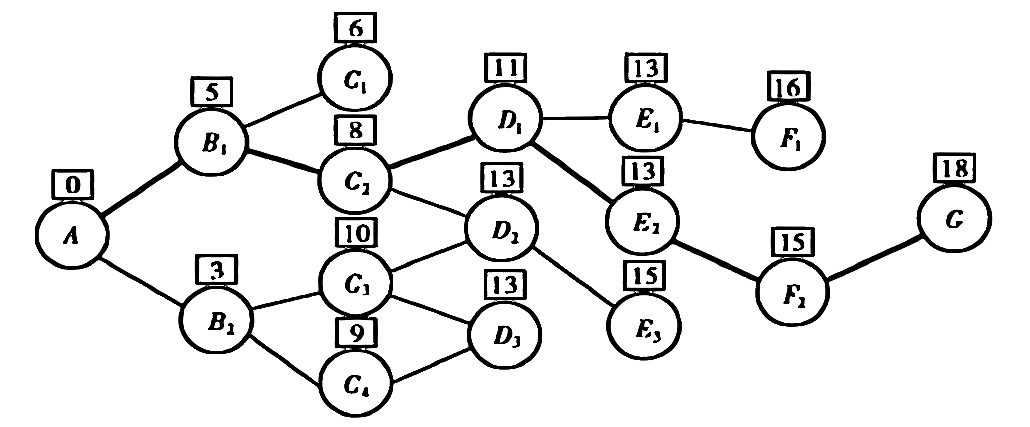
\includegraphics[width=\linewidth]{image/32.png}
        \caption{第七章问题,明显的体现了多阶段概念,比如在B阶段要么B1,要么B2}
    \end{subfigure}
    \hfill
    \begin{subfigure}{0.4\textwidth}
        \centering
        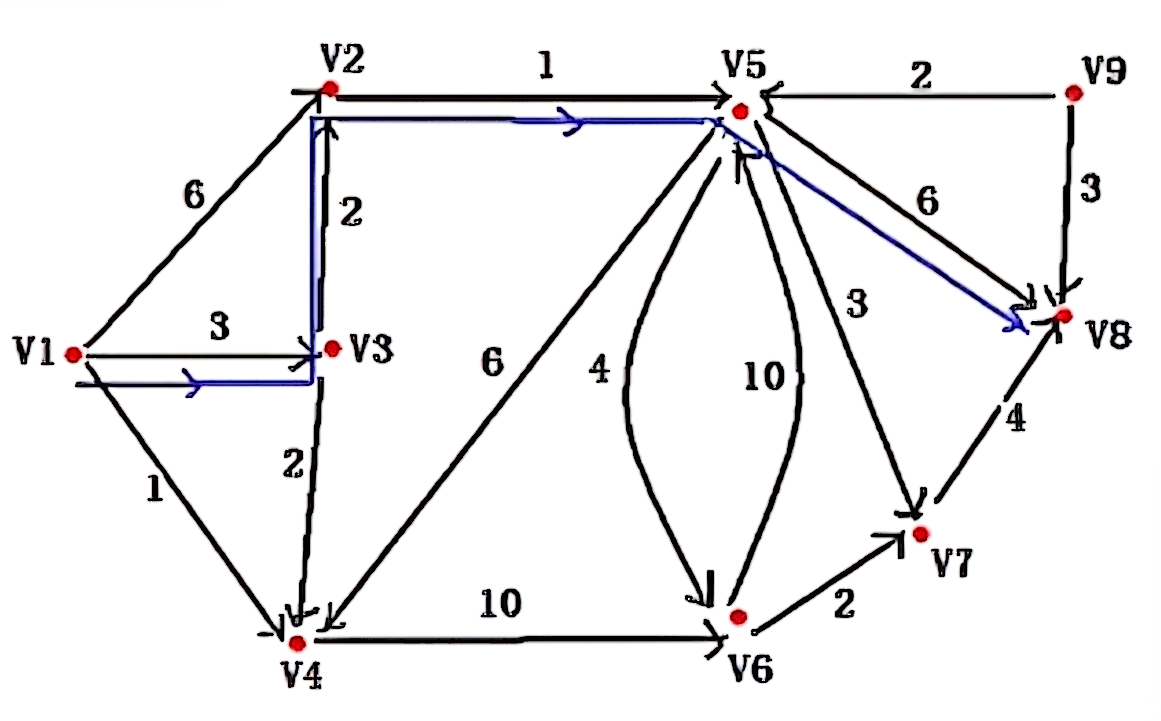
\includegraphics[width=\linewidth]{image/40.png}
        \caption{第九章问题,没有明确的,或者说不强调多阶段概念,是几何图形上的搜索问题,只是要找到最短路径}
    \end{subfigure}
    \caption{动态规划与图论的对比,二者可以说是同源,动态规划更强调多阶段,图论更强调几何选择}
\end{figure}
\ifx\allfiles\undefined
	% 如果有这一部分的参考文献的话,在这里加上
	% 没有的话不需要
	% 因此各个部分的参考文献可以分开放置
	% 也可以统一放在主文件末尾。
	
	%  bibfile.bib是放置参考文献的文件,可以用zotero导出。
	% \bibliography{bibfile}
	
	end{document}
	\else
	\fi